% Copyright (C) Comunidade LaTeX e Gustavo Rodrigues.
% 
% Este é um software livre: você pode redistribuí-lo e/ou modificá-lo
% nos termos da Licença Pública Geral GNU, publicada pela Free Software Foundation,
% versão 3 da Licença ou qualquer versão posterior.
% 
% Você provavelmente recebeu uma cópia da Licença Pública Geral GNU junto com o template. 
% Caso contrário, consulte <http://www.gnu.org/licenses/>.
%
% Criado por Gustavo Silva Rodrigues
% Instruções completas disponíveis em:
% https://github.com/gusirosx/TexTemplate
%===============================================================================================
%                                   Modelo de Tese
%===============================================================================================
\documentclass[12pt,a4paper,oneside]{report}
\usepackage{reffiles/ABNTConfig}
\begin{document}
	% ===== Elementos Pré-Textuais ===== 
	%===============================================================================================
%                                   Elementos Pré-Textuais 
%===============================================================================================
% ====== Capa e Contra Capa ===== 
%===================================================================================================
%                                            CAPA
%===================================================================================================
\begin{titlepage}
	% \pagecolor{blue!10}
	\begin{center}
		\begin{minipage}{2.0cm}
			\begin{center}
				
\includegraphics[width=1.8cm,height=1.8cm]{prefiles/ufu.pdf}	
			\end{center}
		\end{minipage}\hfill
		\begin{minipage}{11.0cm}
			\begin{center}
				\large{\textbf{ UNIVERSIDADE FEDERAL DE UBERLÂNDIA}}\\[0.1cm]
				\large{Faculdade de Engenharia Mecânica}\\[0.1cm]
				%\small{Programa de Pós-Graduação em Engenharia Mecânica}
			\end{center}
		\end{minipage}\hfill
		\begin{minipage}{2.0cm}
			\begin{center}
				
\includegraphics[width=1.8cm,height=1.8cm]{prefiles/mflab.pdf}
			\end{center}
		\end{minipage}
		
		\vspace*{4cm}
		
		\textbf{NOME DO AUTOR}
		
		\vspace{4.5cm}
		{\fontsize{23}{23} \textbf{Título da tese Título da tese Título da tese}}	\\ \vspace{1.2ex}
		{\fontsize{23}{23} \textbf{Título da tese Título da tese}}\\ \vspace{1.2ex}
		%{\fontsize{23}{23} \textbf{Proposta de tese}\\}
		
		\vspace*{11.2cm}
		Uberlândia\\2020
		
	\end{center}
\end{titlepage}
%===================================================================================================
%                                           CONTRA CAPA
%===================================================================================================
\clearpage
\thispagestyle{fancy}
\fancyhf{}
\vspace*{2.5cm}
\begin{center}
	
	{\large \textbf{NOME DO AUTOR}}
	
	\vspace*{2.8cm}
	{\fontsize{23}{23} \textbf{Título da tese Título da tese Título da tese}}	\\ \vspace{1.2ex}
	{\fontsize{23}{23} \textbf{Título da tese Título da tese}}\\ \vspace{1.2ex}
	%{\fontsize{23}{23} \textbf{advectiva-difusiva}}
\end{center}

\vspace*{2.5cm}
\begin{flushright}
	\parbox{3.5in}{ Tese de doutorado apresentada à Faculdade de 
		Engenharia Mecânica da Universidade Federal de Uberlândia como parte dos requisitos exigidos para 
		obtenção do título de Doutor em Engenharia Mecânica.}
\end{flushright}

\vspace{1.0cm}
\noindent
Orientador: Prof. Dr. Nome do Orientador\\
\noindent
Coorientador: Prof. Dr. Nome do Coorientador\\

\vspace{6.5cm}
\begin{center}
	Uberlândia\\2020
\end{center}
%===================================================================================================

% ===== Ficha Catolográfica ===== 
%===================================================================================================
%                                     FICHA CATALOGRÁFICA
%===================================================================================================
\clearpage
\newpage
\thispagestyle{empty}
\vspace*{22.cm}
\noindent Esta página será substituída pela ficha catalográfica da biblioteca.
\clearpage
% ====== Folha de Aprovação ===== 
%===================================================================================================
%                                     FOLHA DE APROVAÇÃO
%===================================================================================================
\clearpage
\begin{center}
	
	%\vspace*{0cm}
	{UNIVERSIDADE FEDERAL DE UBERLÂNDIA\\\vspace{1.2ex}}
	{FACULDADE DE ENGENHARIA MECÂNICA\\\vspace{1.2ex}}

	
	\vspace{1.5cm}
	\textbf{DISSERTAÇÃO DE MESTRADO ACADÊMICO}
	
	\vspace{1.4cm}
	{\fontsize{23}{23} \textbf{Título da tese Título da tese Título da tese}}\\ \vspace{1.2ex}
	{\fontsize{23}{23} \textbf{Título da tese Título da tese}}\\ \vspace{1.2ex}
	\vspace{0.8cm}
	\begin{flushleft}
		\vspace{0.2cm}
		Autor: Nome do Autor\\
		\vspace{0.2cm}
		Orientador: Prof. Dr. Nome do Orientador
		
		\vspace{0.4cm}
		A Banca Examinadora composta pelos membros abaixo aprovou esta Tese:\\
		\vspace{0.5cm}
		\hrulefill\\
		\textbf{Prof. Dr. Nome Completo do Orientador, Presidente\\
			Departamento/Unidade/Instituição \\}
		
		\vspace{0.5cm}
		\hrulefill\\
		\textbf{Prof. Dr. Nome Completo do Membro Interno \\
			Departamento/Unidade/Instituição \\}
		
		\vspace{0.5cm}
		\hrulefill\\
		\textbf{Prof. Dr. Nome Completo do Membro Interno \\
			Departamento/Unidade/Instituição \\}
		\vspace{0.5cm}
		
		\hrulefill\\
		\textbf{Prof. Dr. Nome Completo do Membro Externo \\
			Departamento/Unidade/Instituição \\}
		\vspace{0.5cm}
		
		\hrulefill\\
		\textbf{Prof. Dr. Nome Completo do Membro Externo \\
			Departamento/Unidade/Instituição \\}
		\vspace{0.5cm}
		A ata da defesa com as respectivas assinaturas dos membros encontra-se com a secretária da pós-graduação.
	\end{flushleft}
	
	\begin{flushright}
		\vspace{1.2cm}
		Uberlândia, 20 de abril de 2020.
	\end{flushright}
	
\end{center}
% ========= Dedicatória ========= 
%==============================================================================================
%                                         DEDICATÓRIA
%==============================================================================================
\clearpage
\vspace*{0.75\textheight}
\begin{flushright}
	\textit{Elemento opcional no qual o autor \\ presta homenagem ou dedica seu \\trabalho para uma ou mais pessoas.}
\end{flushright}
% ======= Agradecimentos ======== 
%-------------------------------------------------------------------------------------------
% Tesetex é um software livre: você pode redistribuí-lo e/ou modificá-lo
% nos termos da Licença Pública Geral GNU 3, publicada pela Free Software Foundation.
% Tesetex é distribuído na esperança de que seja útil para você, mas SEM QUALQUER GARANTIA. 
% Veja a Licença Pública Geral GNU para mais detalhes.
% Você provavelmente recebeu uma cópia da Licença Pública Geral GNU junto com o Tesetex. 
% Caso contrário, consulte <http://www.gnu.org/licenses/>.
% Criado por Gustavo Silva Rodrigues e a comunidade LaTeX.
% Instruções completas disponíveis em: https://github.com/gusirosx/Tesetex
%-------------------------------------------------------------------------------------------
%==============================================================================================
%                                       AGRADECIMENTOS
%==============================================================================================
\clearpage
\begin{center}
\chapter*{Agradecimentos}
\end{center}
\vspace*{1cm}
\begin{trivlist}  \itemsep 4ex  \normalsize
%
\item Elemento opcional no qual o autor faz agradecimentos dirigidos àqueles que contribuíram de maneira relevante à elaboração do trabalho.

\item Quando se tratar de dissertações e teses que receberam auxílio financeiro de agências de fomento é recomendada a referência ao apoio recebido.
 
\item O presente trabalho foi realizado com apoio da Coordenação de Aperfeiçoamento de Pessoal de Nível Superior – Brasil (CAPES) – Código de Financiamento 001.

\item O presente trabalho foi realizado com apoio da Conselho Nacional de Desenvolvimento Científico e Tecnológico (CNPq), processo no nnnnnn/aaaa-d.

\item O presente trabalho foi realizado com apoio da Fundação de Amparo à Pesquisa do Estado de Minas Gerais (FAPEMIG), processo aaaa/nnnnn-d.

\item Texto de exemplo, texto de exemplo, texto de exemplo, texto de exemplo, texto de exemplo, texto de exemplo, texto de exemplo, texto de exemplo, texto de exemplo, texto de exemplo, texto de exemplo, texto de exemplo, texto de exemplo, texto de exemplo.

\item Texto de exemplo, texto de exemplo, texto de exemplo, texto de exemplo, texto de exemplo, texto de exemplo, texto de exemplo, texto de exemplo, texto de exemplo, texto de exemplo, texto de exemplo, texto de exemplo, texto de exemplo, texto de exemplo, texto de exemplo.

\end{trivlist}
% ========== Epígrafe =========== 
%-------------------------------------------------------------------------------------------
% Tesetex é um software livre: você pode redistribuí-lo e/ou modificá-lo
% nos termos da Licença Pública Geral GNU 3, publicada pela Free Software Foundation.
% Tesetex é distribuído na esperança de que seja útil para você, mas SEM QUALQUER GARANTIA. 
% Veja a Licença Pública Geral GNU para mais detalhes.
% Você provavelmente recebeu uma cópia da Licença Pública Geral GNU junto com o Tesetex. 
% Caso contrário, consulte <http://www.gnu.org/licenses/>.
% Criado por Gustavo Silva Rodrigues e a comunidade LaTeX.
% Instruções completas disponíveis em: https://github.com/gusirosx/Tesetex
%-------------------------------------------------------------------------------------------
%===================================================================================================
%                                         EPÍGRAFE
%===================================================================================================
\clearpage
\vspace*{6in}
\epigraph{\emph{Parece ser uma das características fundamentais da natureza que as leis físicas fundamentais sejam descritas em termos de uma teoria matemática de grande beleza e poder.}}{Paul Dirac}

% =========== Resumo ============ 
%==============================================================================================
%                                          RESUMO
%==============================================================================================
\clearpage
\begin{center}
	\chapter*{Resumo}
\end{center}
\vspace{24pt}
\onehalfspacing
\noindent
SOBRENOME, Nome. Título da tese Título da tese Título da tese Título da tese Título da tese Título da tese. \pageref{LastPage}p. Tese de Doutorado. Faculdade de Engenharia Mecânica, Universidade Federal de Uberlândia, Uberlândia, 2020.\\

Escreva aqui o texto do seu resumo redigido em parágrafo único, no máximo em uma página, contendo no \textbf{máximo 500 palavras}, apresente um resumo de todos o seu trabalho, incluindo objetivos, metodologia, resultados e conclusões; não inclua apenas a contextualização até chegar nos objetivos, é importante fazer um resumo de todos os capítulos do texto, até chegar à conclusão). Texto de exemplo, texto de exemplo, texto de exemplo, texto de exemplo, texto de exemplo, texto de exemplo, texto de exemplo, texto de exemplo, texto de exemplo, texto de exemplo, texto de exemplo, texto de exemplo, texto de exemplo, texto de exemplo, texto de exemplo, texto de exemplo, texto de exemplo, texto de exemplo, texto de exemplo, texto de exemplo, texto de exemplo, texto de exemplo. Texto de exemplo, texto de exemplo, texto de exemplo, texto de exemplo, texto de exemplo, texto de exemplo, texto de exemplo, texto de exemplo, texto de exemplo, texto de exemplo, texto de exemplo, texto de exemplo, texto de exemplo, texto de exemplo, texto de exemplo, texto de exemplo, texto de exemplo, texto de exemplo, texto de exemplo, texto de exemplo, texto de exemplo, texto de exemplo. Texto de exemplo, texto de exemplo, texto de exemplo, texto de exemplo, texto de exemplo, texto de exemplo, texto de exemplo, texto de exemplo, texto de exemplo, texto de exemplo, texto de exemplo, texto de exemplo, texto de exemplo, texto de exemplo, texto de exemplo, texto de exemplo, texto de exemplo, texto de exemplo, texto de exemplo, texto de exemplo, texto de exemplo, texto de exemplo. Texto de exemplo, texto de exemplo, texto de exemplo, texto de exemplo, texto de exemplo, texto de exemplo, texto de exemplo, texto de exemplo, texto de exemplo, texto de exemplo, texto de exemplo, texto de exemplo, texto de exemplo, texto de exemplo, texto de exemplo, texto de exemplo, texto de exemplo, texto de exemplo, texto de exemplo, texto de exemplo, texto de exemplo, texto de exemplo.
\\
\vspace{1cm}
\noindent
\emph{Palavras-chave}: Palavra1, Palavra2, Palavra3, Palavra4, Palavras5.\\
%==============================================================================================
%                                        ABSTRACT
%==============================================================================================
\clearpage
\begin{center}
	\chapter*{Abstract}
\end{center}
\vspace{24pt}
\noindent
LASTNAME, Name. Thesis title Thesis title Thesis title Thesis title Thesis title Thesis title Thesis title. \pageref{LastPage}p. Ph.D. Thesis. School of Mechanical Engineering, Federal University of Uberlândia, Uberlândia, 2020.\\

Write here the English version of your "Resumo". Example text, example text, example text, example text, example text, example text, example text, example text, example text, example text, example text, example text, example text, example text, example text, example text, example text, example text, example text, example text, example text, example text, example text, example text, example text, example text, example text, example text, example text, example text, example text, example text, example text, example text, example text, example text, example text, example text, example text, example text, example text, example text, example text, example text, example text, example text, example text. Example text, example text, example text, example text, example text, example text, example text, example text, example text, example text, example text, example text, example text, example text, example text, example text, example text, example text, example text, example text, example text, example text.Example text, example text, example text, example text, example text, example text, example text, example text, example text, example text, example text, example text, example text, example text, example text, example text, example text, example text, example text, example text, example text, example text.Example text, example text, example text, example text, example text, example text, example text, example text, example text, example text, example text, example text, example text, example text, example text, example text, example text, example text, example text, example text, example text, example text. Example text, example text, example text, example text, example text, example text, example text, example text, example text, example text, example text, example text, example text, example text, example text, example text, example text, example text, example text, example text, example text, example text example text, example text, example text, example text.
\\

\vspace{1cm}
\noindent
\emph{Keywords}: Keyword1, Keyword2, Keyword3, Keyword4, Keyword5.
% ==== Lista de Ilustrações ===== 
%-------------------------------------------------------------------------------------------
% Tesetex é um software livre: você pode redistribuí-lo e/ou modificá-lo
% nos termos da Licença Pública Geral GNU 3, publicada pela Free Software Foundation.
% Tesetex é distribuído na esperança de que seja útil para você, mas SEM QUALQUER GARANTIA. 
% Veja a Licença Pública Geral GNU para mais detalhes.
% Você provavelmente recebeu uma cópia da Licença Pública Geral GNU junto com o Tesetex. 
% Caso contrário, consulte <http://www.gnu.org/licenses/>.
% Criado por Gustavo Silva Rodrigues e a comunidade LaTeX.
% Instruções completas disponíveis em: https://github.com/gusirosx/Tesetex
%-------------------------------------------------------------------------------------------
%===================================================================================================
%                                    LISTA DE ILUSTRAÇÕES
%===================================================================================================
\clearpage
\phantomsection
\addcontentsline{toc}{chapter}{Lista de Ilustrações}
\renewcommand{\listfigurename}{}{\begin{center} {\chapter*{Lista de Ilustrações}} \end{center}}
\vspace{-13ex}
\listoffigures
% ====== Lista de Tabelas ======= 
%===================================================================================================
%                                    LISTA DE TABELAS
%===================================================================================================
\clearpage
\phantomsection
\addcontentsline{toc}{chapter}{Lista de Tabelas}
\renewcommand{\listtablename}{}
{\begin{center} {\chapter*{Lista de Tabelas}} \end{center}}
\vspace{-13ex}
\listoftables
% ===== Lista de Símbolos ======= 
%===================================================================================================
%                                    LISTA DE SÍMBOLOS
%===================================================================================================
\clearpage
\phantomsection
\addcontentsline{toc}{chapter}{Lista de Abreviaturas e Siglas}
\renewcommand{\listfigurename}
{\begin{center} {\chapter*{Lista de Abreviaturas e Siglas}} \end{center}}
\markboth{Lista de Abreviaturas e Siglas}{Lista de Abreviaturas e Siglas}
\printnomenclature
%===================================================================================================

\begin{center}
\chapter*{Lista de Abreviaturas e Siglas}
\end{center}

\noindent\textbf{\emph{Letras Latinas}}\\

\noindent
\begin{tabular}{l c p{.8\linewidth} c}
	$a_i$ & - & Coeficientes de influencia das equações do momento discretizadas\\
	$A_i$ & - & Coeficientes de influencia modificados \\
	$C$ & - & Constantes \\
	$C_f$ & - & Coeficiente de atrito \\
	$D$ & - & Dilatação, divergente de velocidade \\
	$D_i$ & - & Termo da difusão adimensional\\
	$ER$ & - & Razão de expansão do canal\\
	$F_i$ & - & Fluxo de massa convectiva\\
	$g$ & - & Aceleração gravitacional \\
	$h$ & - & Altura do degrau \\
	$h_E$ & - & Altura do comprimento de entrada do degrau \\
	$H$ & - & Altura total do canal \\
	$L_c$ & - & Comprimento característico\\
	$P$ & - & Pressão física, mais carga hidrostática\\
	$J$ & - & Fluxos viscosos e advectivos combinados através do contorno da célula\\
	$K$ & - & Termo fonte da equação geradora\\
	$Re$ & - & Número de Reynolds\\
	$Pe$ & - & Número de Peclet\\
	$S$ & - & Termo fonte da equação de transporte\\
	$S_a$ & - & Termo fonte da equação de transporte discretizada\\
	$t$ & - & Tempo adimensional\\
	$u$ & - & Componente de velocidade na direção x\\
	$v$ & - & Componente de velocidade na direção y\\
	$V_c$ & - & Velocidade característica\\
	$X_i/h$ & - & Comprimentos característicos de cada região de recirculação\\
\end{tabular}
\newline \newline
\textbf{\emph{Letras Gregas}}\\

\noindent
\begin{tabular}{l c p{.9\linewidth} l}
$\phi$ & - & Variável genérica\\
$\Gamma$ & - & Difusividade\\
$\pi$ & - & Função real para o número de Peclet celular\\
$\Pi$ & - & Coeficientes de influência no esquema de Allen e Southwell\\
$\lambda$ & - & Autovalor da Solução elementar\\
$\chi$ & - & Função real para o número de Peclet celular\\
\end{tabular}
\newline \newline
\begin{tabular}{l c p{.9\linewidth} l}
	$\psi$ & - & Termo de correção para as equações do momentum discretizadas\\
	$\theta$ & - & ângulo entre a malha e o escoamento\\
	$\rho$ & - & Densidade do fluido\\
	$\tau_w$ & - & Tensão de cisalhamento na parede\\
	$\mu$ & - & Viscosidade dinâmica do fluido\\
	$\nu$ & - & Viscosidade cinemática do fluido\\
	$\omega$ & - & Sub-relaxação adotada no método de Gauss-Siedel\\
\end{tabular}
\newline \newline
\textbf{\emph{Siglas}}\\

\noindent
\begin{tabular}{l c p{.8\linewidth} c}
	$\textbf{ADI}$& - & Direção implícita alternada, do inglês \textit{Alternating Direction Implicit} \\
	$\textbf{CDS}$& - & Esquema da diferença central, do inglês \textit{Central Differencing scheme} \\
	$\textbf{CFD}$& - & Dinâmica dos fluidos computacional, do inglês \textit{Computational Fluid Dynamics} \\
	$\textbf{CFL}$& - & \textit{Courant Friedrichs Lewy} \\
	$\textbf{DNS}$& - & Simulações numéricas diretas, do inglês \textit{direct numerical simulations}\\
	$\textbf{FOU}$& - & \textit{Upwind} de primeira ordem, do inglês \textit{First Order Upwind} \\
	$\textbf{LOADS}$& - & Esquema de diferenciação localmente analítico, do inglês \textit{Locally Analytic Differencing Scheme} \\
	$\textbf{MAC}$& - & \textit{Marker and Cell}\\
	$\textbf{MDF}$& - & Métodos das diferenças finitas\\
	$\textbf{MEF}$& - & Métodos dos Elementos Finitos\\
	$\textbf{MVF}$& - & Métodos dos Volumes Finitos\\
	$\textbf{QUICK}$& - & Interpolação quadrática a montante para a cinemática convectiva, do inglês \textit{Quadratic Upstream Interpolation for Convective Kinematics} \\
	$\textbf{QUICKER}$& - & Interpolação quadrática a montante para a cinemática convectiva estendida e revisada, do inglês \textit{Quadratic Upstream Interpolation for Convective Kinematics Extended and Revised}\\
	$\textbf{RMS}$& - & \textit{Root Mean Square} \\
	$\textbf{SIMPLE}$& - & \textit{Semi-Implicit Method for Pressure-Linked Equation} \\
	$\textbf{SIMPLEC}$& - & \textit{Semi-Implicit Method for Pressure-Linked Equation Consistent} \\
	$\textbf{SIMPLER}$& - & \textit{Semi-Implicit Method for Pressure-Linked Equation Revised} \\
	$\textbf{SOU}$& - & \textit{Upwind} de segunda ordem, do inglês \textit{Second Order Upwind} \\
	$\textbf{SOUB}$& - & \textit{Second Order Upwind Biased} \\
	$\textbf{TDMA}$& - & \textit{Tridiagonal Matrix Algorithm} \\
	$\textbf{UNIFAES}$& - & Esquema de abordagem finita unificada do tipo exponencial, do inglês \textit{Unified Finite Approaches Exponential-type Scheme} \\
\end{tabular}
\newline \newline
% =========== Sumário ============ 
%-------------------------------------------------------------------------------------------
% Tesetex é um software livre: você pode redistribuí-lo e/ou modificá-lo
% nos termos da Licença Pública Geral GNU 3, publicada pela Free Software Foundation.
% Tesetex é distribuído na esperança de que seja útil para você, mas SEM QUALQUER GARANTIA. 
% Veja a Licença Pública Geral GNU para mais detalhes.
% Você provavelmente recebeu uma cópia da Licença Pública Geral GNU junto com o Tesetex. 
% Caso contrário, consulte <http://www.gnu.org/licenses/>.
% Criado por Gustavo Silva Rodrigues e a comunidade LaTeX.
% Instruções completas disponíveis em: https://github.com/gusirosx/Tesetex
%-------------------------------------------------------------------------------------------
%===================================================================================================
%                                         Sumário
%===================================================================================================
\clearpage
\phantomsection
\addcontentsline{toc}{chapter}{Sumário}
\renewcommand*\contentsname{}{\begin{center} \chapter*{Sumário} \end{center}}
\vspace{-13ex}
\tableofcontents
\clearpage
%===================================================================================================
%                                    DEMAIS FORMATAÇÕES
%===================================================================================================
\onehalfspacing         % Espaçamento de 1.5
\let\originalchapter=\chapter
\def\chapter{\cleardoublepage\originalchapter}
\setlength{\parskip}{1\baselineskip}
%Comentar esse trecho se quiser omitir a numeração.
%==================================================================================================
\pagestyle{fancy}
\fancyhf{}
\fancyhead[RO,LE]{\thepage}
%==================================================================================================
% ================================ 
	% =========== CAPÍTULO 1 =========== 
	%===================================================================================================
%                                       Capítulo 1 
%===================================================================================================
\chapter{INTRODUÇÃO}\label{cap1}

Este \textit{template} apresenta as regras básicas para a elaboração do trabalho segundo as normas ABNT. Além das regras básicas previstas aqui, solicita-se consultar outros detalhes da norma ABNT sempre que se desejar inserir ou configurar algum elemento não previsto aqui. Ou seja, mesmo que este \textit{template} não preveja as demais regras ABNT, por ser uma visão simplificada, ainda assim elas precisam ser seguidas. 

%---------------------------------------------------------------------------------------------------
\section{Motivação}\label{cap11}

Texto de exemplo, texto de exemplo, texto de exemplo, texto de exemplo, texto de exemplo, texto de exemplo, texto de exemplo, texto de exemplo, texto de exemplo, texto de exemplo, texto de exemplo, texto de exemplo, texto de exemplo, texto de exemplo, texto de exemplo, texto de exemplo, texto de exemplo, texto de exemplo, texto de exemplo, texto de exemplo, texto de exemplo, texto de exemplo, texto de exemplo.

%---------------------------------------------------------------------------------------------------
\section{Objetivos}\label{cap12}

Texto de exemplo, texto de exemplo, texto de exemplo, texto de exemplo, texto de exemplo, texto de exemplo, texto de exemplo, texto de exemplo, texto de exemplo, texto de exemplo, texto de exemplo, texto de exemplo, texto de exemplo, texto de exemplo, texto de exemplo, texto de exemplo, texto de exemplo, texto de exemplo, texto de exemplo, texto de exemplo, texto de exemplo, texto de exemplo, texto de exemplo.Texto de exemplo, texto de exemplo, texto de exemplo, texto de exemplo, texto de exemplo, texto de exemplo, texto de exemplo, texto de exemplo, texto de exemplo, texto de exemplo, texto de exemplo, texto de exemplo, texto de exemplo, texto de exemplo, texto de exemplo, texto de exemplo, texto de exemplo, texto de exemplo, texto de exemplo, texto de exemplo, texto de exemplo, texto de exemplo, texto de exemplo. Texto de exemplo, texto de exemplo, texto de exemplo, texto de exemplo, texto de exemplo, texto de exemplo, texto de exemplo, texto de exemplo, texto de exemplo, texto de exemplo, texto de exemplo, texto de exemplo, texto de exemplo, texto de exemplo, texto de exemplo, texto de exemplo, texto de exemplo, texto de exemplo, texto de exemplo, texto de exemplo, texto de exemplo, texto de exemplo, texto de exemplo.

\section{Justificativa}\label{cap13}


\begin{table}[htbp]
	\centering
	\caption{Exemplo de título de tabela}
	\begin{tabular}{p{1in} p{1in} p{1in} p{1in} } \hline
		
		Cabeçalho 1	& Cabeçalho 2	& Cabeçalho 3	& Cabeçalho 4 \\ \hline
		Texto	& número & número	& número \\ 
		Texto	& número & número	& número \\ 
		Texto	& número & número	& número \\ 
		Texto	& número & número	& número \\ 
		Texto	& número & número	& número \\ \hline
		
	\end{tabular}
	\label{tab:ExemploDeTabela1}
\end{table}


Atenção ao fazer citações a referências para garantir o uso da forma correta, considerando os seguintes exemplos:
\begin{itemize}
	\item Se desejar que uma citação a uma referência apareça no final da frase, use com o comando ``citep''. Exemplo: ``Tal coisa é muito melhor do que aquela outra coisa \citep{Modest2013, Modest2016}''
	\item Se desejar que uma citação a uma referência apareça no meio da frase, como parte da própria frase, use o comando ``citet''. Exemplo: ``De acordo com \citet{Modest2013}, tal coisa é muito melhor do que aquela outra coisa.''
	\item \textbf{Atenção} - nunca usar o comando ``citep'' para citações a referências que aparecem no meio da frase, como parte da própria frase. Exemplo: ``De acordo com \citep{Modest1991}, tal coisa é muito melhor do que aquela outra coisa.''
\end{itemize}

\begin{figure}[!h] 
	\centering
	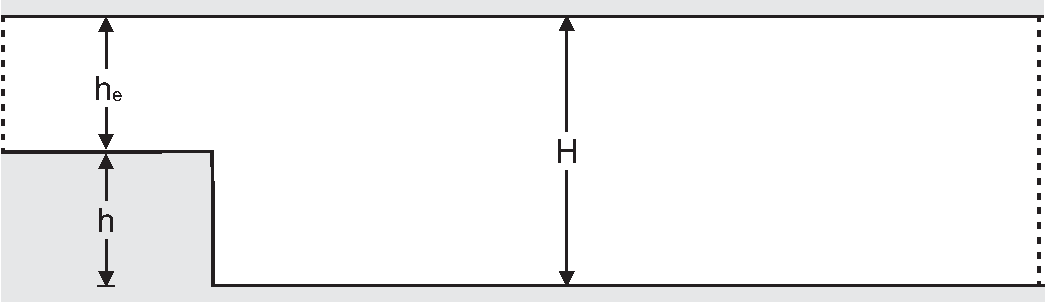
\includegraphics[width=1\textwidth]{./cap1/figs/Canal.pdf}
	\caption{Exemplo de uma figura simples.}
	\label{fig:F2}
\end{figure}

\begin{figure}[!t] 
	\centering
	\subfigure[Solução A]{
		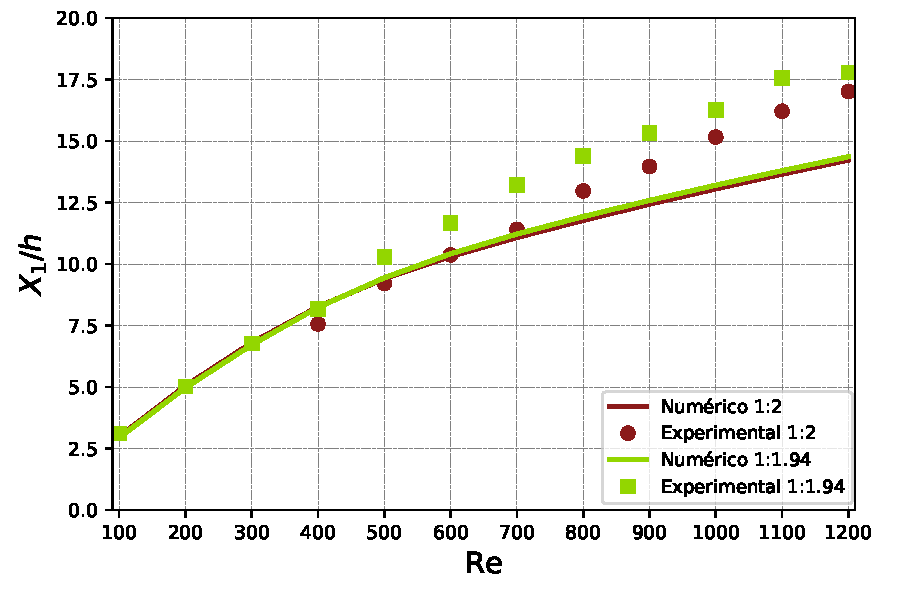
\includegraphics[width=0.45\textwidth]{./cap1/figs/CLAX1.pdf}
		\label{F1A}
	}\hfil
	\subfigure[Solução B]{
		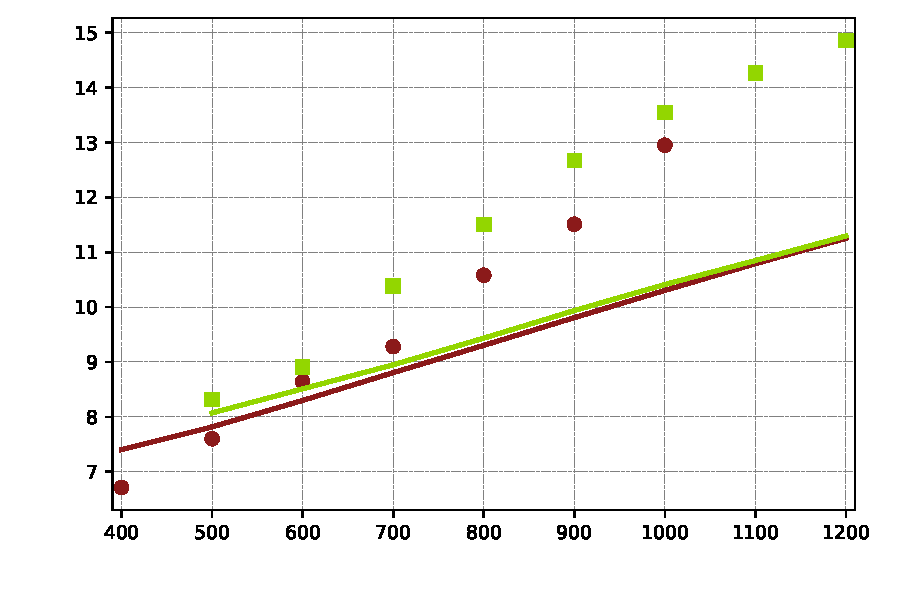
\includegraphics[width=0.45\textwidth]{./cap1/figs/CLAX2.pdf}
		\label{F1B}
	}
	\subfigure[Solução C]{
		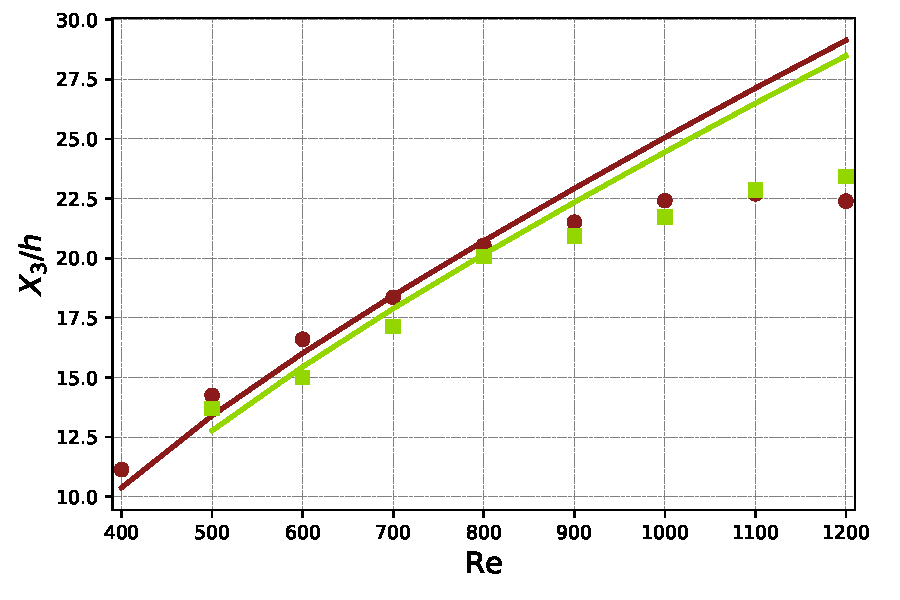
\includegraphics[width=0.45\textwidth]{./cap1/figs/CLAX3.pdf}
		\label{F1C}
	}\hfil
	\subfigure[Solução D]{
		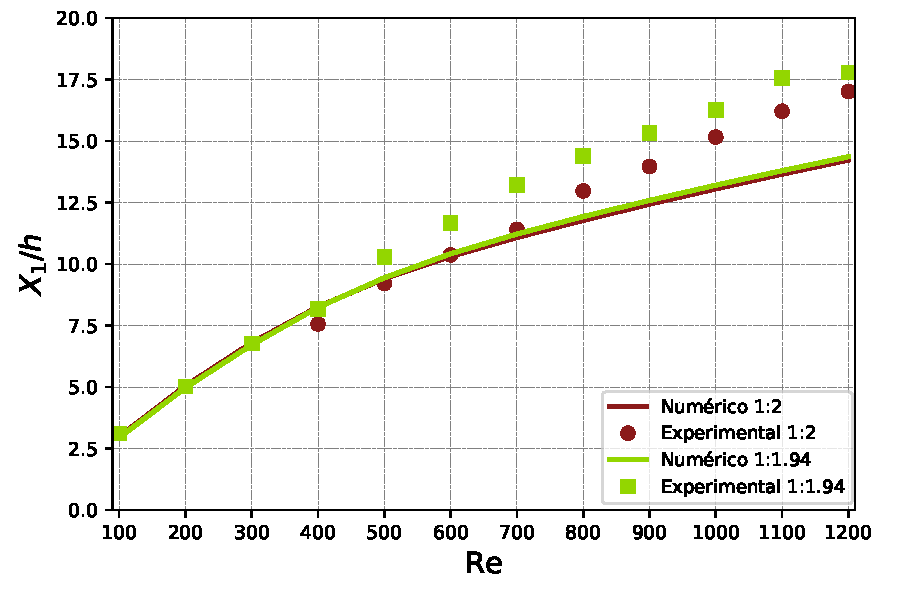
\includegraphics[width=0.45\textwidth]{./cap1/figs/CLAX1.pdf}
		\label{F1D}
	}
	\caption{Exemplo de quatro figuras agrupadas.}
	\label{fig:F1}
\end{figure}



\begin{table}[H]
	\centering
	\caption{Exemplo de Cronograma.}
	\begin{center}
		\begin{tabular}{*{16}{|c} |c|}\hline
			\multirow{2}{*}{Etapas} & \multicolumn{4}{|c|}{2019}& \multicolumn{4}{|c|}{2020}& \multicolumn{4}{|c|}{2021}& \multicolumn{4}{|c|}{2022}\\ \cline{2-17}
			& $1^o$  & $2^o$ & $3^o$ & $4^o$ & $1^o$  & $2^o$  & $3^o$ & $4^o$ & $1^o$  & $2^o$ & $3^o$ & $4^o$ & $1^o$  & $2^o$  & $3^o$ & $4^o$ \\\hline
			A & x & x & x & x & x & x & x & x & x & x & x & x & x & x & x & x  \\\hline
			B & x & x & x & x &   &   &   &   &   &   &   &   &   &   &   &   \\\hline
			C &   &   & x & x & x &   &   &   &   &   &   &   &   &   &   &   \\\hline
			D &   &   &   &   & x & x & x & x &   &   &   &   &   &   &   &   \\\hline
			E &   &   &   &   &   &   & x & x & x & x &   &   &   &   &   &   \\\hline
			F &   &   &   &   &   &   &   & x & x & x & x & x &   &   &   &   \\\hline
			G &   &   &   &   &   &   &   &   & x & x & x & x &   &   &   &   \\\hline
			H &   &   &   &   &   &   &   &   &   & x & x & x & x &   &   &   \\\hline
			I &   &   &   &   &   &   &   &   &   &   &   & x & x & x & x & x  \\\hline
			J &   &   &   &   &   &   &   &   &   &   &   & x & x & x & x & x \\\hline
			K &   &   &   &   &   & x &   & x &   & x &   & x &   & x &   & x  \\\hline
			L &   &   &   &   &   &   &   &   &   & x & x & x & x & x & x & x  \\\hline
		\end{tabular}
		\label{tab:crono}
	\end{center}
\end{table}
	% =========== CAPÍTULO 2 =========== 
	%===================================================================================================
%                                       Capítulo 2 
%===================================================================================================
\chapter{REVISÃO BIBLIOGRÁFICA}\label{cap2}

Texto de exemplo, texto de exemplo, texto de exemplo, texto de exemplo, texto de exemplo, texto de exemplo, texto de exemplo, texto de exemplo, texto de exemplo, texto de exemplo, texto de exemplo, texto de exemplo, texto de exemplo, texto de exemplo, texto de exemplo, texto de exemplo, texto de exemplo, texto de exemplo, texto de exemplo, texto de exemplo, texto de exemplo, texto de exemplo, texto de exemplo.Texto de exemplo, texto de exemplo, texto de exemplo, texto de exemplo, texto de exemplo, texto de exemplo, texto de exemplo, texto de exemplo, texto de exemplo, texto de exemplo, texto de exemplo, texto de exemplo, texto de exemplo, texto de exemplo, texto de exemplo, texto de exemplo, texto de exemplo, texto de exemplo, texto de exemplo, texto de exemplo, texto de exemplo, texto de exemplo, texto de exemplo. Texto de exemplo, texto de exemplo, texto de exemplo, texto de exemplo, texto de exemplo, texto de exemplo, texto de exemplo, texto de exemplo, texto de exemplo, texto de exemplo, texto de exemplo, texto de exemplo, texto de exemplo, texto de exemplo, texto de exemplo, texto de exemplo, texto de exemplo, texto de exemplo, texto de exemplo, texto de exemplo, texto de exemplo, texto de exemplo, texto de exemplo.

%---------------------------------------------------------------------------------------------------
\section{Aspectos Práticos}\label{cap21}

Texto de exemplo, texto de exemplo, texto de exemplo, texto de exemplo, texto de exemplo, texto de exemplo, texto de exemplo, texto de exemplo, texto de exemplo, texto de exemplo, texto de exemplo, texto de exemplo, texto de exemplo, texto de exemplo, texto de exemplo, texto de exemplo, texto de exemplo, texto de exemplo, texto de exemplo, texto de exemplo, texto de exemplo, texto de exemplo, texto de exemplo.Texto de exemplo, texto de exemplo, texto de exemplo, texto de exemplo, texto de exemplo, texto de exemplo, texto de exemplo, texto de exemplo, texto de exemplo, texto de exemplo, texto de exemplo, texto de exemplo, texto de exemplo, texto de exemplo, texto de exemplo, texto de exemplo, texto de exemplo, texto de exemplo, texto de exemplo, texto de exemplo, texto de exemplo, texto de exemplo, texto de exemplo. Texto de exemplo, texto de exemplo, texto de exemplo, texto de exemplo, texto de exemplo, texto de exemplo, texto de exemplo, texto de exemplo, texto de exemplo, texto de exemplo, texto de exemplo, texto de exemplo, texto de exemplo, texto de exemplo, texto de exemplo, texto de exemplo, texto de exemplo, texto de exemplo, texto de exemplo, texto de exemplo, texto de exemplo, texto de exemplo, texto de exemplo.

%---------------------------------------------------------------------------------------------------




	% =========== CAPÍTULO 3 =========== 
	%===================================================================================================
%                                       Capítulo 3 
%===================================================================================================
\chapter{FUNDAMENTAÇÃO TEÓRICA}\label{cap3}

Texto de exemplo, texto de exemplo, texto de exemplo, texto de exemplo, texto de exemplo, texto de exemplo, texto de exemplo, texto de exemplo, texto de exemplo, texto de exemplo, texto de exemplo, texto de exemplo, texto de exemplo, texto de exemplo, texto de exemplo, texto de exemplo, texto de exemplo, texto de exemplo, texto de exemplo, texto de exemplo, texto de exemplo, texto de exemplo, texto de exemplo.Texto de exemplo, texto de exemplo, texto de exemplo, texto de exemplo, texto de exemplo, texto de exemplo, texto de exemplo, texto de exemplo, texto de exemplo, texto de exemplo, texto de exemplo, texto de exemplo, texto de exemplo, texto de exemplo, texto de exemplo, texto de exemplo, texto de exemplo, texto de exemplo, texto de exemplo, texto de exemplo, texto de exemplo, texto de exemplo, texto de exemplo. Texto de exemplo, texto de exemplo, texto de exemplo, texto de exemplo, texto de exemplo, texto de exemplo, texto de exemplo, texto de exemplo, texto de exemplo, texto de exemplo, texto de exemplo, texto de exemplo, texto de exemplo, texto de exemplo, texto de exemplo, texto de exemplo, texto de exemplo, texto de exemplo, texto de exemplo, texto de exemplo, texto de exemplo, texto de exemplo, texto de exemplo.

%---------------------------------------------------------------------------------------------------
\section{Motivação}\label{cap31}

Texto de exemplo, texto de exemplo, texto de exemplo, texto de exemplo, texto de exemplo, texto de exemplo, texto de exemplo, texto de exemplo, texto de exemplo, texto de exemplo, texto de exemplo, texto de exemplo, texto de exemplo, texto de exemplo, texto de exemplo, texto de exemplo, texto de exemplo, texto de exemplo, texto de exemplo, texto de exemplo, texto de exemplo, texto de exemplo, texto de exemplo.Texto de exemplo, texto de exemplo, texto de exemplo, texto de exemplo, texto de exemplo, texto de exemplo, texto de exemplo, texto de exemplo, texto de exemplo, texto de exemplo, texto de exemplo, texto de exemplo, texto de exemplo, texto de exemplo, texto de exemplo, texto de exemplo, texto de exemplo, texto de exemplo, texto de exemplo, texto de exemplo, texto de exemplo, texto de exemplo, texto de exemplo. Texto de exemplo, texto de exemplo, texto de exemplo, texto de exemplo, texto de exemplo.
%---------------------------------------------------------------------------------------------------





	% =========== CAPÍTULO 4 =========== 
	%===================================================================================================
%                                       Capítulo 4 
%===================================================================================================
\chapter{Metodologia e Aplicações}\label{cap4}

A descrição das técnicas utilizadas deve ser precisa e clara permitindo ao leitor a compreensão do trabalho, e tornar possível que outros pesquisadores repitam na íntegra o mesmo método.

	% =========== CAPÍTULO 5 =========== 
	%===================================================================================================
%                                       Capítulo 5 
%===================================================================================================
\chapter{RESULTADOS E DISCUSSÕES}\label{cap5}

Texto de exemplo, texto de exemplo, texto de exemplo, texto de exemplo, texto de exemplo, texto de exemplo, texto de exemplo, texto de exemplo, texto de exemplo, texto de exemplo, texto de exemplo, texto de exemplo, texto de exemplo, texto de exemplo, texto de exemplo, texto de exemplo, texto de exemplo, texto de exemplo, texto de exemplo, texto de exemplo, texto de exemplo, texto de exemplo, texto de exemplo.Texto de exemplo, texto de exemplo, texto de exemplo, texto de exemplo, texto de exemplo, texto de exemplo, texto de exemplo, texto de exemplo, texto de exemplo, texto de exemplo, texto de exemplo, texto de exemplo, texto de exemplo, texto de exemplo, texto de exemplo, texto de exemplo, texto de exemplo, texto de exemplo, texto de exemplo, texto de exemplo, texto de exemplo, texto de exemplo, texto de exemplo. Texto de exemplo, texto de exemplo, texto de exemplo, texto de exemplo, texto de exemplo, texto de exemplo, texto de exemplo, texto de exemplo, texto de exemplo, texto de exemplo, texto de exemplo, texto de exemplo, texto de exemplo, texto de exemplo, texto de exemplo, texto de exemplo, texto de exemplo, texto de exemplo, texto de exemplo, texto de exemplo, texto de exemplo, texto de exemplo, texto de exemplo.

\section{title}
\subsection{title}
\subsubsection{title}
	% =========== CAPÍTULO 6 =========== 
	%===================================================================================================
%                                       Capítulo 6 
%===================================================================================================
\chapter{CONCLUSÕES}\label{cap6}

Texto de exemplo, texto de exemplo, texto de exemplo, texto de exemplo, texto de exemplo, texto de exemplo, texto de exemplo, texto de exemplo, texto de exemplo, texto de exemplo, texto de exemplo, texto de exemplo, texto de exemplo, texto de exemplo, texto de exemplo, texto de exemplo, texto de exemplo, texto de exemplo, texto de exemplo, texto de exemplo, texto de exemplo, texto de exemplo, texto de exemplo.Texto de exemplo, texto de exemplo, texto de exemplo, texto de exemplo, texto de exemplo, texto de exemplo, texto de exemplo, texto de exemplo, texto de exemplo, texto de exemplo, texto de exemplo, texto de exemplo, texto de exemplo, texto de exemplo, texto de exemplo, texto de exemplo, texto de exemplo, texto de exemplo, texto de exemplo, texto de exemplo, texto de exemplo, texto de exemplo, texto de exemplo. Texto de exemplo, texto de exemplo, texto de exemplo, texto de exemplo, texto de exemplo, texto de exemplo, texto de exemplo, texto de exemplo, texto de exemplo, texto de exemplo, texto de exemplo, texto de exemplo, texto de exemplo, texto de exemplo, texto de exemplo, texto de exemplo, texto de exemplo, texto de exemplo, texto de exemplo, texto de exemplo, texto de exemplo, texto de exemplo, texto de exemplo.





	% ========== Referências =========== 
	%===================================================================================================
%                                       Referências
%===================================================================================================
\clearpage
\phantomsection
\addcontentsline{toc}{chapter}{REFERÊNCIAS BIBLIOGRÁFICAS}
\DeclareRobustCommand{\refname}{\begin{center} REFERÊNCIAS BIBLIOGRÁFICAS \end{center} \vspace*{1.8cm}}
\bibliographystyle{reffiles/bibconfig}
\bibliography{reffiles/bibliografia}
	% =========== Apêndices ============ 
	%-------------------------------------------------------------------------------------------
% Tesetex é um software livre: você pode redistribuí-lo e/ou modificá-lo
% nos termos da Licença Pública Geral GNU 3, publicada pela Free Software Foundation.
% Tesetex é distribuído na esperança de que seja útil para você, mas SEM QUALQUER GARANTIA. 
% Veja a Licença Pública Geral GNU para mais detalhes.
% Você provavelmente recebeu uma cópia da Licença Pública Geral GNU junto com o Tesetex. 
% Caso contrário, consulte <http://www.gnu.org/licenses/>.
% Criado por Gustavo Silva Rodrigues e a comunidade LaTeX.
% Instruções completas disponíveis em: https://github.com/gusirosx/Tesetex
%-------------------------------------------------------------------------------------------
%===============================================================================================
%                                   Apêndices
%===============================================================================================
\phantomsection
\addcontentsline{toc}{chapter}{Apêndices}
%===============================================================================================
% ========= Apêndice A ===========
\renewcommand{\thechapter}{A}
%===================================================================================================
%                                          Apêndice A
%===================================================================================================
\begin{center}
	\appendix{-- \ \ Primeiro Apêndice}\label{ApendiceA}
\end{center}

Texto ou documento elaborado pelo autor, a fim de complementar sua argumentação, sem prejuízo da unidade nuclear do trabalho.

Texto de exemplo, texto de exemplo, texto de exemplo, texto de exemplo, texto de exemplo, texto de exemplo, texto de exemplo, texto de exemplo, texto de exemplo, texto de exemplo, texto de exemplo, texto de exemplo, texto de exemplo, texto de exemplo, texto de exemplo, texto de exemplo, texto de exemplo, texto de exemplo, texto de exemplo, texto de exemplo, texto de exemplo, texto de exemplo, texto de exemplo.Texto de exemplo, texto de exemplo, texto de exemplo, texto de exemplo, texto de exemplo, texto de exemplo, texto de exemplo, texto de exemplo, texto de exemplo, texto de exemplo, texto de exemplo, texto de exemplo, texto de exemplo, texto de exemplo, texto de exemplo, texto de exemplo, texto de exemplo, texto de exemplo, texto de exemplo, texto de exemplo, texto de exemplo, texto de exemplo, texto de exemplo. Texto de exemplo, texto de exemplo, texto de exemplo, texto de exemplo, texto de exemplo, texto de exemplo, texto de exemplo, texto de exemplo, texto de exemplo, texto de exemplo, texto de exemplo, texto de exemplo, texto de exemplo, texto de exemplo, texto de exemplo, texto de exemplo, texto de exemplo, texto de exemplo, texto de exemplo, texto de exemplo, texto de exemplo, texto de exemplo, texto de exemplo.

%==========================================================================================================
\clearpage   
% ========= Apêndice B ===========
\renewcommand{\thechapter}{B}
%===================================================================================================
%                                          Apêndice B
%===================================================================================================
\begin{center}
	\appendix{-- \ \ Segundo Apêndice}\label{ApendiceB}
\end{center}

Texto de exemplo, texto de exemplo, texto de exemplo, texto de exemplo, texto de exemplo, texto de exemplo, texto de exemplo, texto de exemplo, texto de exemplo, texto de exemplo, texto de exemplo, texto de exemplo, texto de exemplo, texto de exemplo, texto de exemplo, texto de exemplo, texto de exemplo, texto de exemplo, texto de exemplo, texto de exemplo, texto de exemplo, texto de exemplo, texto de exemplo.Texto de exemplo, texto de exemplo, texto de exemplo, texto de exemplo, texto de exemplo, texto de exemplo, texto de exemplo, texto de exemplo, texto de exemplo, texto de exemplo, texto de exemplo, texto de exemplo, texto de exemplo, texto de exemplo, texto de exemplo, texto de exemplo, texto de exemplo, texto de exemplo, texto de exemplo, texto de exemplo, texto de exemplo, texto de exemplo, texto de exemplo. Texto de exemplo, texto de exemplo, texto de exemplo, texto de exemplo, texto de exemplo, texto de exemplo, texto de exemplo, texto de exemplo, texto de exemplo, texto de exemplo, texto de exemplo, texto de exemplo, texto de exemplo, texto de exemplo, texto de exemplo, texto de exemplo, texto de exemplo, texto de exemplo, texto de exemplo, texto de exemplo, texto de exemplo, texto de exemplo, texto de exemplo.




%==========================================================================================================  
   
	% ============ Anexos ============== 
	%===============================================================================================
%                                          Anexos
%===============================================================================================
\newpage
\let\originalanexo=\anexo
\def\appendix{\cleardoublepage\originalanexo}
\setcounter{chapter}{0}
\def\thechapter{\Alph{chapter}}
\phantomsection
\addcontentsline{toc}{chapter}{ANEXOS}
%===============================================================================================
% ========== Anexo A ============
%===================================================================================================
%                                           Anexo A
%===================================================================================================
\begin{center}
	\anexo{-- \ \ Primeiro Anexo}\label{Anexo A}
\end{center}

Texto ou documento não elaborado pelo autor, que serve de fundamentação, comprovação e ilustração.

Texto de exemplo, texto de exemplo, texto de exemplo, texto de exemplo, texto de exemplo, texto de exemplo, texto de exemplo, texto de exemplo, texto de exemplo, texto de exemplo, texto de exemplo, texto de exemplo, texto de exemplo, texto de exemplo, texto de exemplo, texto de exemplo, texto de exemplo, texto de exemplo, texto de exemplo, texto de exemplo, texto de exemplo, texto de exemplo, texto de exemplo.Texto de exemplo, texto de exemplo, texto de exemplo, texto de exemplo, texto de exemplo, texto de exemplo, texto de exemplo, texto de exemplo, texto de exemplo, texto de exemplo, texto de exemplo, texto de exemplo, texto de exemplo, texto de exemplo, texto de exemplo, texto de exemplo, texto de exemplo, texto de exemplo, texto de exemplo, texto de exemplo, texto de exemplo, texto de exemplo, texto de exemplo. Texto de exemplo, texto de exemplo, texto de exemplo, texto de exemplo, texto de exemplo, texto de exemplo, texto de exemplo, texto de exemplo, texto de exemplo, texto de exemplo, texto de exemplo, texto de exemplo, texto de exemplo, texto de exemplo, texto de exemplo, texto de exemplo, texto de exemplo, texto de exemplo, texto de exemplo, texto de exemplo, texto de exemplo, texto de exemplo, texto de exemplo.
%===================================================================================================
\clearpage   
% ========== Anexo B ============
%===================================================================================================
%                                           Anexo B
%===================================================================================================
\begin{center}
	\anexo{-- \ \ Segundo Anexo}\label{Anexo B}
\end{center}

Texto de exemplo, texto de exemplo, texto de exemplo, texto de exemplo, texto de exemplo, texto de exemplo, texto de exemplo, texto de exemplo, texto de exemplo, texto de exemplo, texto de exemplo, texto de exemplo, texto de exemplo, texto de exemplo, texto de exemplo, texto de exemplo, texto de exemplo, texto de exemplo, texto de exemplo, texto de exemplo, texto de exemplo, texto de exemplo, texto de exemplo.Texto de exemplo, texto de exemplo, texto de exemplo, texto de exemplo, texto de exemplo, texto de exemplo, texto de exemplo, texto de exemplo, texto de exemplo, texto de exemplo, texto de exemplo, texto de exemplo, texto de exemplo, texto de exemplo, texto de exemplo, texto de exemplo, texto de exemplo, texto de exemplo, texto de exemplo, texto de exemplo, texto de exemplo, texto de exemplo, texto de exemplo. Texto de exemplo, texto de exemplo, texto de exemplo, texto de exemplo, texto de exemplo, texto de exemplo, texto de exemplo, texto de exemplo, texto de exemplo, texto de exemplo, texto de exemplo, texto de exemplo, texto de exemplo, texto de exemplo, texto de exemplo, texto de exemplo, texto de exemplo, texto de exemplo, texto de exemplo, texto de exemplo, texto de exemplo, texto de exemplo, texto de exemplo.
%===================================================================================================
\clearpage  
% ===============================







 
	% ================================== 
\end{document}
